

\section{Intermediate Representation}

Spatial programs are internally represented in the compiler as a hierarchical dataflow graph (DFG).
Nodes in this graph represent control structures, data operations, and memory allocations, while edges represent data and effect dependencies.
Nesting of controllers directly translates to the hierarchy in the intermediate representation.
Design parameters are kept as graph metadata, such that they can be independently updated without changing the graph itself.

\newsavebox{\gemm}
\begin{lrbox}{\gemm}
\begin{lstlisting}[language=Spatial,linewidth=0.4\textwidth]
// Load data from files
val a = loadMatrix[Float](args(0))
val b = loadMatrix[Float](args(1))

// Allocate space on accelerator DRAM
val A = DRAM[Float](a.rows,a.cols)
val B = DRAM[Float](b.rows,b.cols)
val C = DRAM[Float](a.rows,b.cols)

// Create explicit design parameters
val M = 128 (64, 1024)  // Tile size - rows
val N = 128 (64, 1024)  // Tile size - cols
val P = 128 (64, 1024)  // Tile size - common
val PAR_K  = 2 (1, 8)   // Unroll factor of k
val PAR_J  = 2 (1, 16)  // Unroll factor of j

// Transfer data to accelerator DRAM
sendMatrix(A, a)
sendMatrix(B, b)

// Specify the accelerator design
Accel {
  // Produce C in M x N tiles
  Foreach(A.rows by M, B.cols by N){
    (ii,jj) =>
    val tileC = SRAM[Float](M, N)
    // Combine intermediates (outer)
    MemReduce(tileC)(A.cols by P){ kk =>
      // Allocate on-chip scratchpads
      val tileA = SRAM[Float](M, P)
      val tileB = SRAM[Float](P, N)
      val accum = SRAM[Float](M, N)

      // Load tiles of A and B from DRAM
      tileA load A(ii::ii+M, kk::kk+P)
      tileB load B(kk::kk+P, jj::jj+N)

      // Combine intermediates (across P)
      MemReduce(accum)(P par PAR_K){ k =>
        val partC = SRAM[Float](M, N)
        Foreach(M by 1, N par PAR_J){ (i,j) =>
          partC(i,j) = tileA(i,k) * tileB(k,j)
        }
        partC
      // Combine with element-wise add
      }{(a,b) => a + b }
    }{(a,b) => a + b }

    // Store the tile of C to DRAM
    C(ii::ii+M, jj::jj+N) store tileC
  }
}
// Save the result to another file
saveMatrix(args(2), getMatrix(C))
\end{lstlisting}
\end{lrbox}

\begin{figure}
\begin{tabular}{cm{0.4\textwidth}m{0.6\textwidth}}
{\hspace{10pt}\usebox{\gemm}} &
{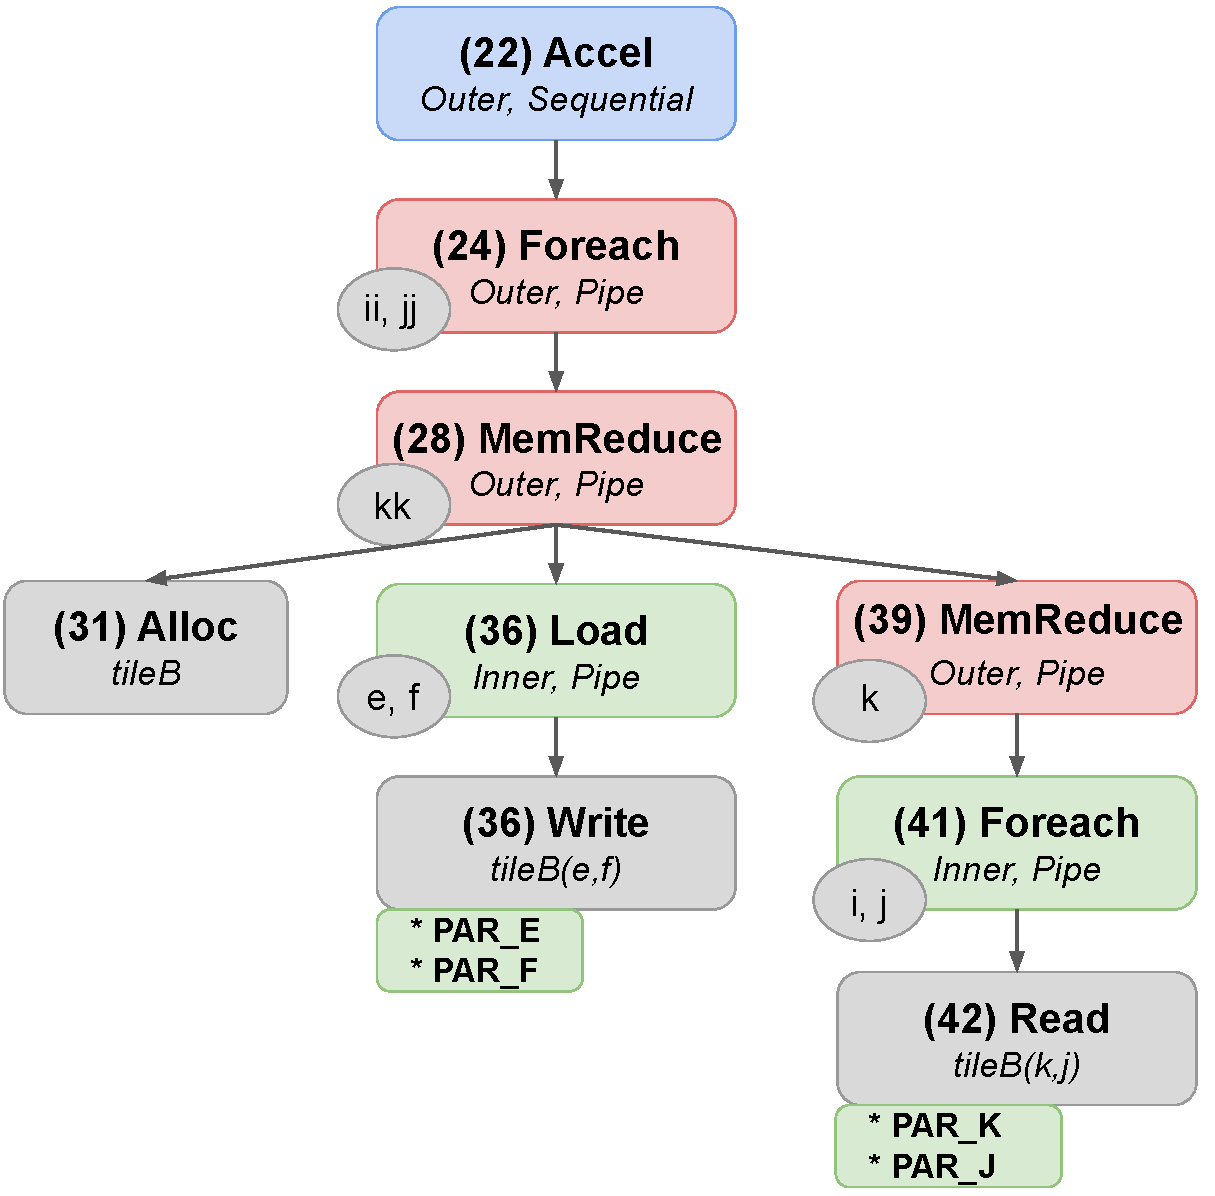
\includegraphics[width=0.55\textwidth]{5-compiler/figs/ctrltree.pdf}} \\
{\parbox{0.4\textwidth}{\centering{a. Spatial implementation. }}} &
{\parbox{0.6\textwidth}{\centering{b. Control/access tree for \texttt{\small{tileB}}.}}}
\end{tabular} %% end resizebox
\caption{Matrix multiplication ($C$~=~$A~\cdot~B$) implemented in Spatial and corresponding control/access tree IR. Control nodes are annotated with their control level, schedule, and loop iterator name. Outer sequential nodes are blue, outer pipeline nodes are red, and inner pipelined control nodes are green. Memory access nodes (gray) are annotated with their parallelization factor.}
\label{fig:matmult}
\end{figure}


When discussing DFG transformations and optimizations, it is often useful to think about the graph as a controller/access tree. Figure~\ref{fig:matmult} shows an example of one such controller tree for the memory {\texttt{\small{tileB}} in the Spatial code example of matrix multiplication. Note that transfers between on-chip and off-chip memory each expand to a control node which linearly accesses the on-chip memory, in this case by iterators \texttt{e} and \texttt{f}.
This tree abstracts away most primitive operations, leaving only relevant controller hierarchy and the memory
accesses for a specific memory.

Within the acceleratable subset of Spatial, nodes are formally separated into three categories:
control nodes, memory allocation nodes, and primitive nodes.
Control nodes represent state machine structures like \texttt{\small{Foreach}} and \texttt{\small{Reduce}} described in Chapter~\ref{controls}.
Primitive nodes are operations which may consume, but never produce, control signals, including on-chip memory accesses.
Primitive nodes are further broken down into ``physical'' operations requiring resources and ``ephemeral'' operations which are only used for bookkeeping purposes in the compiler. For example, bit selects and grouping of words into structs require no hardware resources but are used to track necessary wires in the generated code.
